\documentclass[10pt]{beamer}

\usepackage{hyperref}
\usepackage{graphicx}
\usepackage{times}

\usepackage{fancyvrb}
\usepackage{color}

\title{Introduction to Programming with Python}
\subtitle{Riding the Serpent}
\author{Anshul Nigham \& Rob Tirrell}
\date{\today}


\usetheme{Luebeck}
\hypersetup{
  pdftitle = \title,
  pdfauthor = {Rob Tirrell},
  pdfsubject = {Introduction to Programming with Python},
  colorlinks = true,
  urlcolor=blue
}

% Get rid of bottom navigation bars.
\setbeamertemplate{footline}[page number]{}

% Get rid of navigation symbols.
\setbeamertemplate{navigation symbols}{}

\makeatletter
\def\PY@reset{\let\PY@it=\relax \let\PY@bf=\relax%
    \let\PY@ul=\relax \let\PY@tc=\relax%
    \let\PY@bc=\relax \let\PY@ff=\relax}
\def\PY@tok#1{\csname PY@tok@#1\endcsname}
\def\PY@toks#1+{\ifx\relax#1\empty\else%
    \PY@tok{#1}\expandafter\PY@toks\fi}
\def\PY@do#1{\PY@bc{\PY@tc{\PY@ul{%
    \PY@it{\PY@bf{\PY@ff{#1}}}}}}}
\def\PY#1#2{\PY@reset\PY@toks#1+\relax+\PY@do{#2}}

\def\PY@tok@gd{\def\PY@tc##1{\textcolor[rgb]{0.63,0.00,0.00}{##1}}}
\def\PY@tok@gu{\let\PY@bf=\textbf\def\PY@tc##1{\textcolor[rgb]{0.50,0.00,0.50}{##1}}}
\def\PY@tok@gt{\def\PY@tc##1{\textcolor[rgb]{0.00,0.25,0.82}{##1}}}
\def\PY@tok@gs{\let\PY@bf=\textbf}
\def\PY@tok@gr{\def\PY@tc##1{\textcolor[rgb]{1.00,0.00,0.00}{##1}}}
\def\PY@tok@cm{\let\PY@it=\textit\def\PY@tc##1{\textcolor[rgb]{0.25,0.50,0.50}{##1}}}
\def\PY@tok@vg{\def\PY@tc##1{\textcolor[rgb]{0.10,0.09,0.49}{##1}}}
\def\PY@tok@m{\def\PY@tc##1{\textcolor[rgb]{0.40,0.40,0.40}{##1}}}
\def\PY@tok@mh{\def\PY@tc##1{\textcolor[rgb]{0.40,0.40,0.40}{##1}}}
\def\PY@tok@go{\def\PY@tc##1{\textcolor[rgb]{0.50,0.50,0.50}{##1}}}
\def\PY@tok@ge{\let\PY@it=\textit}
\def\PY@tok@vc{\def\PY@tc##1{\textcolor[rgb]{0.10,0.09,0.49}{##1}}}
\def\PY@tok@il{\def\PY@tc##1{\textcolor[rgb]{0.40,0.40,0.40}{##1}}}
\def\PY@tok@cs{\let\PY@it=\textit\def\PY@tc##1{\textcolor[rgb]{0.25,0.50,0.50}{##1}}}
\def\PY@tok@cp{\def\PY@tc##1{\textcolor[rgb]{0.74,0.48,0.00}{##1}}}
\def\PY@tok@gi{\def\PY@tc##1{\textcolor[rgb]{0.00,0.63,0.00}{##1}}}
\def\PY@tok@gh{\let\PY@bf=\textbf\def\PY@tc##1{\textcolor[rgb]{0.00,0.00,0.50}{##1}}}
\def\PY@tok@ni{\let\PY@bf=\textbf\def\PY@tc##1{\textcolor[rgb]{0.60,0.60,0.60}{##1}}}
\def\PY@tok@nl{\def\PY@tc##1{\textcolor[rgb]{0.63,0.63,0.00}{##1}}}
\def\PY@tok@nn{\let\PY@bf=\textbf\def\PY@tc##1{\textcolor[rgb]{0.00,0.00,1.00}{##1}}}
\def\PY@tok@no{\def\PY@tc##1{\textcolor[rgb]{0.53,0.00,0.00}{##1}}}
\def\PY@tok@na{\def\PY@tc##1{\textcolor[rgb]{0.49,0.56,0.16}{##1}}}
\def\PY@tok@nb{\def\PY@tc##1{\textcolor[rgb]{0.00,0.50,0.00}{##1}}}
\def\PY@tok@nc{\let\PY@bf=\textbf\def\PY@tc##1{\textcolor[rgb]{0.00,0.00,1.00}{##1}}}
\def\PY@tok@nd{\def\PY@tc##1{\textcolor[rgb]{0.67,0.13,1.00}{##1}}}
\def\PY@tok@ne{\let\PY@bf=\textbf\def\PY@tc##1{\textcolor[rgb]{0.82,0.25,0.23}{##1}}}
\def\PY@tok@nf{\def\PY@tc##1{\textcolor[rgb]{0.00,0.00,1.00}{##1}}}
\def\PY@tok@si{\let\PY@bf=\textbf\def\PY@tc##1{\textcolor[rgb]{0.73,0.40,0.53}{##1}}}
\def\PY@tok@s2{\def\PY@tc##1{\textcolor[rgb]{0.73,0.13,0.13}{##1}}}
\def\PY@tok@vi{\def\PY@tc##1{\textcolor[rgb]{0.10,0.09,0.49}{##1}}}
\def\PY@tok@nt{\let\PY@bf=\textbf\def\PY@tc##1{\textcolor[rgb]{0.00,0.50,0.00}{##1}}}
\def\PY@tok@nv{\def\PY@tc##1{\textcolor[rgb]{0.10,0.09,0.49}{##1}}}
\def\PY@tok@s1{\def\PY@tc##1{\textcolor[rgb]{0.73,0.13,0.13}{##1}}}
\def\PY@tok@sh{\def\PY@tc##1{\textcolor[rgb]{0.73,0.13,0.13}{##1}}}
\def\PY@tok@sc{\def\PY@tc##1{\textcolor[rgb]{0.73,0.13,0.13}{##1}}}
\def\PY@tok@sx{\def\PY@tc##1{\textcolor[rgb]{0.00,0.50,0.00}{##1}}}
\def\PY@tok@bp{\def\PY@tc##1{\textcolor[rgb]{0.00,0.50,0.00}{##1}}}
\def\PY@tok@c1{\let\PY@it=\textit\def\PY@tc##1{\textcolor[rgb]{0.25,0.50,0.50}{##1}}}
\def\PY@tok@kc{\let\PY@bf=\textbf\def\PY@tc##1{\textcolor[rgb]{0.00,0.50,0.00}{##1}}}
\def\PY@tok@c{\let\PY@it=\textit\def\PY@tc##1{\textcolor[rgb]{0.25,0.50,0.50}{##1}}}
\def\PY@tok@mf{\def\PY@tc##1{\textcolor[rgb]{0.40,0.40,0.40}{##1}}}
\def\PY@tok@err{\def\PY@bc##1{\fcolorbox[rgb]{1.00,0.00,0.00}{1,1,1}{##1}}}
\def\PY@tok@kd{\let\PY@bf=\textbf\def\PY@tc##1{\textcolor[rgb]{0.00,0.50,0.00}{##1}}}
\def\PY@tok@ss{\def\PY@tc##1{\textcolor[rgb]{0.10,0.09,0.49}{##1}}}
\def\PY@tok@sr{\def\PY@tc##1{\textcolor[rgb]{0.73,0.40,0.53}{##1}}}
\def\PY@tok@mo{\def\PY@tc##1{\textcolor[rgb]{0.40,0.40,0.40}{##1}}}
\def\PY@tok@kn{\let\PY@bf=\textbf\def\PY@tc##1{\textcolor[rgb]{0.00,0.50,0.00}{##1}}}
\def\PY@tok@mi{\def\PY@tc##1{\textcolor[rgb]{0.40,0.40,0.40}{##1}}}
\def\PY@tok@gp{\let\PY@bf=\textbf\def\PY@tc##1{\textcolor[rgb]{0.00,0.00,0.50}{##1}}}
\def\PY@tok@o{\def\PY@tc##1{\textcolor[rgb]{0.40,0.40,0.40}{##1}}}
\def\PY@tok@kr{\let\PY@bf=\textbf\def\PY@tc##1{\textcolor[rgb]{0.00,0.50,0.00}{##1}}}
\def\PY@tok@s{\def\PY@tc##1{\textcolor[rgb]{0.73,0.13,0.13}{##1}}}
\def\PY@tok@kp{\def\PY@tc##1{\textcolor[rgb]{0.00,0.50,0.00}{##1}}}
\def\PY@tok@w{\def\PY@tc##1{\textcolor[rgb]{0.73,0.73,0.73}{##1}}}
\def\PY@tok@kt{\def\PY@tc##1{\textcolor[rgb]{0.69,0.00,0.25}{##1}}}
\def\PY@tok@ow{\let\PY@bf=\textbf\def\PY@tc##1{\textcolor[rgb]{0.67,0.13,1.00}{##1}}}
\def\PY@tok@sb{\def\PY@tc##1{\textcolor[rgb]{0.73,0.13,0.13}{##1}}}
\def\PY@tok@k{\let\PY@bf=\textbf\def\PY@tc##1{\textcolor[rgb]{0.00,0.50,0.00}{##1}}}
\def\PY@tok@se{\let\PY@bf=\textbf\def\PY@tc##1{\textcolor[rgb]{0.73,0.40,0.13}{##1}}}
\def\PY@tok@sd{\let\PY@it=\textit\def\PY@tc##1{\textcolor[rgb]{0.73,0.13,0.13}{##1}}}

\def\PYZbs{\char`\\}
\def\PYZus{\char`\_}
\def\PYZob{\char`\{}
\def\PYZcb{\char`\}}
\def\PYZca{\char`\^}
% for compatibility with earlier versions
\def\PYZat{@}
\def\PYZlb{[}
\def\PYZrb{]}
\makeatother



\begin{document}

\begin{frame}
  \titlepage
\end{frame}

\begin{frame}
  \small
  \frametitle{About Us}
  \begin{block}{Anshul Nigham}
    \begin{itemize}
      \item Works somewhere and does something.
      \item Look, it's relevant.
      \item And he's qualified! :)
    \end{itemize}
  \end{block}
  \begin{block}{Rob Tirrell}
    \begin{itemize}
      \item Second-year grad student in Biomedical Informatics here at Stanford.
      \item Works in the Butte lab (\href{http://buttelab.stanford.edu/}{http://buttelab.stanford.edu/}), an entirely 'dry' lab (computers only -- the only other equipment necessary is a coffee machine).
      \item First language was Python, spends most days writing code in R, Python, Ruby and C++.
    \end{itemize}
  \end{block}
\end{frame}

\begin{frame}
  \frametitle{What is Python?}
  \centering
  
\includegraphics[scale=0.5]{PythonLogo.png} \\
  \begin{itemize}
    \item First released in 1991 by a Dutchman named Guido van Rossum (GvR).
    \item That's Self-Appointed Benevolent Dictator for Life (SABDFL) van Rossum to the rest of us.
    \item An interpreted, high-level language with flexible typing.
    \item Currently on its third major release... in other words, very mature.
  \end{itemize}
\end{frame}

\begin{frame}
  \frametitle{A Satisfied User}
  \small
  \begin{quote}
      ``Python has been an important part of Google since the beginning, and remains so as the system grows and evolves. Today dozens of Google engineers use Python, and we're looking for more people with skills in this language.''
  \end{quote}
  \begin{flushright}
    -- Peter Norvig, Director of Search Quality at Google and Computer Science Superstar
  \end{flushright}
\end{frame}

\begin{frame}
  \frametitle{Other Satisfied Users}
  \begin{itemize}
    \item \textbf{AstraZeneca} uses Python in drug discovery pipelines.
    \item \textbf{Phillips'} fabrication plants are managed in Python.
    \item \textbf{Industrial Light \& Magic} (Star Wars) employs Python for process management.
    \item In \textbf{Rob's} work, people use Python at every point in the research pipeline (preprocessing and sanitization, standard analyses, data aggregation and integration, and so forth).
    \item It may be new to you, but according to TIOBE's programming languages index, Python is the sixth-most popular in the world.
    \item A list of anecdotes can't quite prove a point, so we'll try to justify why you should care about and use Python.
  \end{itemize}
\end{frame}

\begin{frame}
  \frametitle{Good for Them, What's in it for You?}
  \begin{block}{Power}
    \begin{itemize}
      \item Python facilitates rapid development.
        It comes with a huge collection of software (libraries) for many purposes.
      \item There is a large, vibrant Python community/ecosystem.
    \end{itemize}
  \end{block}
  \begin{block}{Clarity}
    \begin{itemize}
      \item Python is remarkably clear and readable compared to many other languages.
      \item It actually takes some effort to write difficult-to-understand programs.
    \end{itemize}
  \end{block}
\end{frame}

\begin{frame}
  \frametitle{Datatypes (1)}
  \begin{block}{What are They?}
    \begin{itemize}
      \item A \textbf{datatype} refers to a location in the computer's memory and the type of information stored there.
      \item Numbers can be of the \texttt{int} (integer) datatype, like \texttt{4}, or the \texttt{float} (floating point) datatype, like \texttt{4.0}).
      \item Text uses the \texttt{string} datatype, like \texttt{'Four score and seven years ago...'}.
      \item True and false values are \texttt{bool} (boolean) datatypes, in Python these are \texttt{True} and \texttt{False}.
        There is also a special value called \texttt{None}, that indicates 'no value'.
      \item We can view the type of any variable using \texttt{type}, so \texttt{type('bananagram')} is \texttt{$<$type 'string'$>$}.
    \end{itemize}
  \end{block}
\end{frame}

\begin{frame}[fragile]
  \frametitle{Datatypes (2)}
  \begin{block}{More Advanced Datatypes}
    \begin{itemize}
      \item Obviously, more complex programs require more complex datatypes (depending on the complexity, they may be referred to as 'data structures').
      \item The two most important in Python are the \texttt{list} and \texttt{dict} (dictionary).
      \item A list: 
\begin{Verbatim}[commandchars=\\\{\}]
\PY{n}{some\PYZus{}list} \PY{o}{=} \PY{p}{[}\PY{l+m+mi}{12}\PY{p}{,} \PY{l+s}{'}\PY{l+s}{monkeys}\PY{l+s}{'}\PY{p}{]}
\end{Verbatim}
      \item A dictionary:
\begin{Verbatim}[commandchars=\\\{\}]
\PY{n}{some\PYZus{}dict} \PY{o}{=} \PY{p}{\PYZob{}}
  \PY{l+s}{'}\PY{l+s}{New York}\PY{l+s}{'}\PY{p}{:} \PY{l+s}{'}\PY{l+s}{A state in the US.}\PY{l+s}{'}\PY{p}{,} 
  \PY{l+m+mi}{42}\PY{p}{:} \PY{l+s}{'}\PY{l+s}{A completely irrelevant number.}\PY{l+s}{'}\PY{p}{,} 
  \PY{l+s}{'}\PY{l+s}{today\PYZus{}is\PYZus{}sunday}\PY{l+s}{'}\PY{p}{:} \PY{n}{False}
\PY{p}{\PYZcb{}}
\end{Verbatim}
    \end{itemize}
  \end{block}
\end{frame}

\begin{frame}[fragile]
  \frametitle{Datatypes (3)}
  \begin{block}{Duck Typing}
    \begin{itemize}
      \item The Python philosophy: if it looks like a duck, and it quacks like a duck, then it's a duck.
      \item In other words, variables are not restricted to contain a particular datatype.
        We can re-assign them to anything we want:
        \footnotesize
\begin{Verbatim}[commandchars=\\\{\}]
\PY{n}{var} \PY{o}{=} \PY{l+m+mi}{44}
\PY{n}{var} \PY{o}{=} \PY{l+s}{'}\PY{l+s}{The Life of Brian}\PY{l+s}{'}
\PY{n}{var} \PY{o}{=} \PY{p}{[}
  \PY{l+s}{'}\PY{l+s}{Episode IV: A New Hope}\PY{l+s}{'}\PY{p}{,} 
  \PY{l+s}{'}\PY{l+s}{Episode V: The Empire Strikes Back}\PY{l+s}{'}\PY{p}{,} 
  \PY{l+s}{'}\PY{l+s}{Episode VI: Return of the Jedi}\PY{l+s}{'}
\PY{p}{]}
\PY{n}{var} \PY{o}{=} \PY{p}{\PYZob{}}
  \PY{l+s}{'}\PY{l+s}{aardvark}\PY{l+s}{'}\PY{p}{:} \PY{l+s}{'}\PY{l+s}{a nocturnal burrower from Africa}\PY{l+s}{'}\PY{p}{,}
  \PY{l+s}{'}\PY{l+s}{antbear}\PY{l+s}{'}\PY{p}{:} \PY{l+s}{'}\PY{l+s}{another name for an aardvark}\PY{l+s}{'}
\PY{p}{\PYZcb{}}
\end{Verbatim}
        \normalsize
      \item Functions exist to coerce strings like \texttt{'1024'} into the corresponding floating-point or integer numbers (c.f. \texttt{int()} and \texttt{float()}), or numbers into the corresponding string (c.f. \texttt{str()}), and so on.
    \end{itemize}
  \end{block}
\end{frame}

\begin{frame}[fragile]
  \frametitle{Datatypes (4)}
  \begin{block}{Rolling Our Own Classes}
    \begin{itemize}
      \item We can also write custom classes with the \texttt{class} keyword, with which we can define datatypes (or data structures) that store arbitrary and have a set of methods to manipulate that data.
        \footnotesize
\begin{Verbatim}[commandchars=\\\{\}]
\PY{k}{class} \PY{n+nc}{MyTestClass}\PY{p}{:}
  \PY{k}{def} \PY{n+nf}{\PYZus{}\PYZus{}init\PYZus{}\PYZus{}}\PY{p}{(}\PY{n+nb+bp}{self}\PY{p}{,} \PY{n}{name}\PY{p}{)}\PY{p}{:}
    \PY{n+nb+bp}{self}\PY{o}{.}\PY{n}{name} \PY{o}{=} \PY{n}{name}
  \PY{k}{def} \PY{n+nf}{say\PYZus{}hello}\PY{p}{(}\PY{n+nb+bp}{self}\PY{p}{,} \PY{n}{other\PYZus{}name}\PY{p}{)}\PY{p}{:}
    \PY{k}{print} \PY{n+nb+bp}{self}\PY{o}{.}\PY{n}{name} \PY{o}{+} \PY{l+s}{'}\PY{l+s}{ says hi to }\PY{l+s}{'} \PY{o}{+} \PY{n}{other\PYZus{}name}
\PY{n}{my\PYZus{}test\PYZus{}class\PYZus{}instance} \PY{o}{=} \PY{n}{MyTestClass}\PY{p}{(}\PY{l+s}{'}\PY{l+s}{Rocko}\PY{l+s}{'}\PY{p}{)}
\PY{n}{my\PYZus{}test\PYZus{}class\PYZus{}instance}\PY{o}{.}\PY{n}{say\PYZus{}hello}\PY{p}{(}\PY{l+s}{'}\PY{l+s}{Clarissa}\PY{l+s}{'}\PY{p}{)}
\PY{c}{# >>> 'Rocko says hi to Clarissa'}
\end{Verbatim}
      \normalsize
      \item The ability to extend the language with our own classes is extremely useful, but for concerns of time we'll just dangle the idea in front of you and leave it that.
        Any book on Python will have a more thorough discussion of classes.
    \end{itemize}
  \end{block}
\end{frame}
      

\begin{frame}[fragile]
  \frametitle{Introduction to Functions and Methods (1)}
  \begin{block}{Making Things Happen}
    \begin{itemize}
      \item \textbf{Functions} and \textbf{methods}\footnote{There is a difference: methods are attached to and operate on their objects, while functions stand alone. e.g., \texttt{say\_hello} in the class on the preceding page was a \texttt{method} associated with \texttt{MyTestClass} objects. Don't worry too much about this now, we'll come back to it later (and in this course will only write functions, anyway).} are procedures that work on variables to transform or otherwise alter them.
      \item Change a string to all uppercase:
\begin{Verbatim}[commandchars=\\\{\}]
\PY{n}{some\PYZus{}string} \PY{o}{=} \PY{l+s}{'}\PY{l+s}{julius}\PY{l+s}{'}
\PY{n}{some\PYZus{}string} \PY{o}{=} \PY{n}{some\PYZus{}string}\PY{o}{.}\PY{n}{upper}\PY{p}{(}\PY{p}{)}
\PY{n}{some\PYZus{}string}
\PY{c}{# >>> 'JULIUS'}
\end{Verbatim}
      \item Access an entry (sometimes called an element) of a dictionary:
\begin{Verbatim}[commandchars=\\\{\}]
\PY{n}{some\PYZus{}dict}\PY{p}{[}\PY{l+m+mi}{42}\PY{p}{]}
\PY{c}{# >>> 'A completely irrelevant number'}
\end{Verbatim}
    \end{itemize}
  \end{block}
\end{frame}

\begin{frame}[fragile]
  \frametitle{Introduction to Functions and Methods (2)}
  \begin{block}{A Few More Examples}
    \begin{itemize}
      \item Many of Python's datatypes support this sort of access (called indexing).
\begin{Verbatim}[commandchars=\\\{\}]
\PY{n}{some\PYZus{}string}\PY{p}{[}\PY{l+m+mi}{1}\PY{p}{]}
\PY{c}{# >>> 'U'}
\end{Verbatim}
      \item This is an important point: in Python, the first element of a collection is the \texttt{[0]}th'' one, available at \texttt{collection[0]}.
      \item Similarly, for lists:
\begin{Verbatim}[commandchars=\\\{\}]
\PY{n}{some\PYZus{}list}\PY{p}{[}\PY{l+m+mi}{1}\PY{p}{]}
\PY{c}{# >>> 'monkey'}
\end{Verbatim}
    \end{itemize}
  \end{block}
\end{frame}

\begin{frame}
  \frametitle{The Interpreter (1)}
  \begin{block}{$>>>$}
    \begin{itemize}
      \item As Python is an interpreted language (the computer reads, understands (compiles) and executes it on the fly, instead of reading and compiling ahead of time (as with C, C++, and many others).
      \item Because of this, we can use Python interactively, which is extremely helpful for designing and troubleshooting code.
    \end{itemize}
  \end{block}
  \begin{block}{IDLE}
    \begin{itemize}
      \item IDLE is Python's interpreter shell, which we'll use to walk through examples throughout the course.
      \item For those of you with Macs, you can open a Terminal and launch Python by typing \texttt{python}.
    \end{itemize}
  \end{block}
\end{frame}

\begin{frame}[fragile]
  \frametitle{The Interpreter (2)}
  \begin{block}{The \texttt{print} Function}
    \begin{itemize}
      \item Strings are surrounded by single (') or double (``) quotes, which are equivalent (but you must use the same type for any particular string).
        e.g., if you want a string to have a contraction \texttt{"mustn't"}, you can use double quotes to surround it, like \texttt{"The white whale mustn't breach, Moby is waiting."}.
      \item \texttt{print} is a core Python function, which by default outputs text to the screen. It's somewhat special, in that parentheses are optional when using (calling) it.
    \end{itemize}
  \end{block}
  \begin{block}{A Longstanding Tradition}
      Three equivalent \texttt{'Hello, World!'}:
\begin{Verbatim}[commandchars=\\\{\}]
\PY{k}{print} \PY{l+s}{'}\PY{l+s}{Hello, World!}\PY{l+s}{'}
\PY{k}{print} \PY{l+s}{"}\PY{l+s}{Hello, World!}\PY{l+s}{"}
\PY{k}{print}\PY{p}{(}\PY{l+s}{'}\PY{l+s}{Hello, World!}\PY{l+s}{'}\PY{p}{)}
\end{Verbatim}
  \end{block}
\end{frame}

\begin{frame}
  \frametitle{Brief Interlude: Setting Up KomodoEdit}
  \begin{center}
    
\includegraphics[width=240px]{KomodoEdit.png}
  \end{center}
  KomodoEdit should already be installed on the provided computers, if not, visit \href{http://www.activestate.com/komodo-edit/downloads}{http://www.activestate.com/komodo-edit/downloads} to grab it.
\end{frame}

\begin{frame}[fragile]
  \frametitle{Functions (1)}
  \begin{block}{Writing Your Own with \texttt{def}}
    \begin{itemize}
      \item The \texttt{def} keyword is used to create new functions.
      \item Functions always \texttt{return} a value. 
        Functions which do not explicitly \texttt{return} a value (have no \texttt{return} statement) implicitly return \texttt{None}.
        \small
\begin{Verbatim}[commandchars=\\\{\}]
\PY{c}{# This function has no parameters and...}
\PY{k}{def} \PY{n+nf}{test\PYZus{}func\PYZus{}1}\PY{p}{(}\PY{p}{)}\PY{p}{:}
  \PY{k}{print} \PY{l+s}{"}\PY{l+s}{I}\PY{l+s}{'}\PY{l+s}{m useless!}\PY{l+s}{"}
\end{Verbatim}
    \end{itemize}
  \end{block}
\end{frame}

\begin{frame}[fragile]
  \frametitle{Functions (2)}
\small
\begin{Verbatim}[commandchars=\\\{\}]
\PY{c}{# This function has no parameters and returns None.}
\PY{k}{def} \PY{n+nf}{test\PYZus{}func\PYZus{}2}\PY{p}{(}\PY{p}{)}\PY{p}{:}
  \PY{k}{pass}

\PY{c}{# This function has one parameter - a number.}
\PY{c}{# It adds 10 and returns that value.}
\PY{k}{def} \PY{n+nf}{add\PYZus{}10}\PY{p}{(}\PY{n}{parameter\PYZus{}1}\PY{p}{)}\PY{p}{:}
  \PY{k}{return} \PY{n}{parameter\PYZus{}1} \PY{o}{+} \PY{l+m+mi}{10}
\end{Verbatim}
  \begin{block}{Write Your Own}
    Try writing a simple function that takes one parameter (a string) and uses \texttt{+} to display \texttt{'Hello $<$your string goes here$>$'}.
  \end{block}
\end{frame}

\begin{frame}[fragile]
  \frametitle{Igpay Atinlay (1)}
  \begin{block}{Pig Latin}
    Pig latin is a nonsense language, that can be generated easily for any English word, by moving the word's first character to the end and adding \texttt{'ay'}.
    Then, \texttt{pig\_latinize('pork') = 'orkpay'}
  \end{block}
  \begin{block}{String Indexing and Slicing}
    \begin{itemize}
      \item Recall that we can access single elements of a collection using \texttt{[]}.
        We can also access longer parts of the string (which is a collection of characters) using \textbf{slices}.
\begin{Verbatim}[commandchars=\\\{\}]
\PY{n}{green\PYZus{}eggs} \PY{o}{=} \PY{l+s}{'}\PY{l+s}{green eggs and ham}\PY{l+s}{'}
\PY{k}{print} \PY{n}{green\PYZus{}eggs}\PY{p}{[}\PY{l+m+mi}{6}\PY{p}{:}\PY{l+m+mi}{10}\PY{p}{]}
\PY{o}{>>}\PY{o}{>} \PY{l+s}{'}\PY{l+s}{eggs}\PY{l+s}{'}
\end{Verbatim}
      \item Slices range from \texttt{0}, the first element, to \texttt{-1}, the last element.
      \item Omitting the start or end defaults to 'from the beginning' or 'to the end', respectively.
        Thus, \texttt{some\_collection[:] == some\_collection}.
    \end{itemize}
  \end{block}
\end{frame}

\begin{frame}[fragile]
  \frametitle{Igpay Atinlay (2)}
  \begin{block}{Reading User Input with \texttt{raw\_input}}
    \begin{itemize}
      \item Often, we'll want to get input from a user (e.g., a name).
      \item The \texttt{raw\_input} function does exactly that.
        We pass it one argument, a string that will be printed as the prompt (e.g. \texttt{'Enter your name: '}).
      \item It returns whatever the user enters in response\footnote{The \texttt{'\textbackslash'} just allows us to continue a Python expression on the next line, so it doesn't run off of the slide :).}:
\begin{Verbatim}[commandchars=\\\{\}]
\PY{n}{favorite\PYZus{}color} \PY{o}{=} \PYZbs{}
  \PY{n+nb}{raw\PYZus{}input}\PY{p}{(}\PY{l+s}{'}\PY{l+s}{What is your favourite color? }\PY{l+s}{'}\PY{p}{)}
\end{Verbatim}
        Then \texttt{favorite\_color} will be \texttt{'red'}, or \texttt{'Black'}, etc..
    \end{itemize}
  \end{block}
\end{frame}


\begin{frame}[fragile]
  \frametitle{Igpay Atinlay (3)}
  \begin{block}{Make Your Own Nonsense}
    \begin{itemize}
      \item Using slicing, write a function that takes one parameter (a string) and returns the pig latinized version of the string.
      \item We'll have to make one slice, access one element of the string directly, and then add 'ay' at the end:
        \texttt{$<$all but the first character$>$ + $<$the first character$>$ + 'ay'}.
    \end{itemize}
  \end{block}
\end{frame}

\begin{frame}
  \frametitle{Igpay Atinlay versus igPay atinLay (4)}
  \begin{block}{Improving Pig Latinization}
    You probably noticed that capitalized characters look out of place in the first version of the function.
    There are two string methods, \texttt{lower} and \texttt{capitalize}\footnote{An exhaustive list of string methods is available at \href{http://docs.python.org/library/string.html}{http://docs.python.org/library/string.html}.  All of the builtin libraries are well-documented, see \href{http://docs.python.org}{http://docs.python.org}}, that we can use to fix this problem.
    \begin{itemize}
      \item Modify the function so that it converts the pig latinized string to lowercase, then capitalizes it.
      \item We can do all of this in one line, but it is easier to read and understand if you store the intermediate pig latinized string in its own variables, like \texttt{pig\_latinized\_string}.
      \item Helpfully, we can 'chain' method calls, in other words, \texttt{some\_string.lower().capitalize()} works!
    \end{itemize}
  \end{block}
\end{frame}

\begin{frame}[fragile]
  \frametitle{Dealing with Uncertainty (1)}
  \begin{block}{Truth Testing}
    \begin{itemize}
      \item Few programs are just a straight pipeline of unbiased transformations to data -- most of the time, we'll want to branch out and make decisions based on input.
      \item Python has the \texttt{if}, \texttt{elif} and \texttt{else} keywords that provide this ability.
\begin{Verbatim}[commandchars=\\\{\}]
\PY{n}{some\PYZus{}boolean} \PY{o}{=} \PY{n}{true}
\PY{k}{if} \PY{n}{some\PYZus{}boolean}\PY{p}{:}
  \PY{k}{print} \PY{l+s}{'}\PY{l+s}{Truly today is a special day!}\PY{l+s}{'}
\PY{k}{else}\PY{p}{:}
  \PY{k}{print} \PY{l+s}{'}\PY{l+s}{Back to the grind, peasant.}\PY{l+s}{'}
\end{Verbatim}
    \end{itemize}
  \end{block}
\end{frame}
      
\begin{frame}[fragile]
  \frametitle{Dealing with Uncertainty (2)}
  \begin{block}{Equality}
    \begin{itemize}
      \item We can also use \texttt{==}, \texttt{$<$}, \texttt{$<$=}, and so on.
      \item The instructions following an \texttt{elif} keyword are only triggered if no previous conditions are met and the \texttt{elif} condition is.
\begin{Verbatim}[commandchars=\\\{\}]
\PY{n}{strength} \PY{o}{=} \PY{l+m+mi}{15}
\PY{k}{if} \PY{n}{strength} \PY{o}{>}\PY{o}{=} \PY{l+m+mi}{15}\PY{p}{:}
  \PY{k}{print} \PY{l+s}{'}\PY{l+s}{You pull the sword from the stone.}\PY{l+s}{'}
  \PY{k}{print} \PY{l+s}{'}\PY{l+s}{All hail King Arthur!}\PY{l+s}{'}
\PY{k}{elif} \PY{n}{strength} \PY{o}{>}\PY{o}{=} \PY{l+m+mi}{10}\PY{p}{:}
  \PY{k}{print} \PY{l+s}{'}\PY{l+s}{Solid effort.}\PY{l+s}{'}
  \PY{k}{print} \PY{l+s}{'}\PY{l+s}{But you were born to work in the mines.}\PY{l+s}{'}
\PY{k}{else}\PY{p}{:}
  \PY{k}{print} \PY{l+s}{'}\PY{l+s}{Nope! Not even close.}\PY{l+s}{'}
\end{Verbatim}
      Looks like it's deep, dark and dirty for this guy.
    \end{itemize}
  \end{block}
\end{frame}
    
\begin{frame}
  \frametitle{Case Study: The Candy Shoppe (1)}
  \begin{block}{A Profitable Business Proposition}
    \begin{itemize}
      \item You run a candy shoppe, selling all variety of popsticks, licorice screamers, fireballs and the like.
      \item Little kids are big business you, and these little sugar fiends are spending their parents money and are not very sensitive to changes in price.
        Being a businessperson first and foremost concerned with the bottom line, you want to charge anyone less than \texttt{14} years old a little bit extra (\texttt{25\%} over regular price).
      \item But you're not a monster, and if the customer's blood sugar is below \texttt{2.5}, you'll give him or her a \texttt{15\%} discount (with no additional penalty for being less than \texttt{14}).
      \item You want this to be done transparently, so you will add a function to your cash machine that jacks up the price depending on the customer's information (which is stored in the customer's loyalty card).
    \end{itemize}
  \end{block}
\end{frame}

\begin{frame}[fragile]
  \frametitle{Case Study: The Candy Shoppe (2)}
  \begin{block}{Customer Information}
    \begin{itemize}
      \item Each customer's loyalty card has several attributes encoded in the magstripe.
      \item These attributes are loaded into the cash machine when you scan the card, and are available to the software as a dictionary.
\begin{Verbatim}[commandchars=\\\{\}]
\PY{n}{customer\PYZus{}info} \PY{o}{=} \PY{p}{\PYZob{}}
  \PY{l+s}{'}\PY{l+s}{name}\PY{l+s}{'}\PY{p}{:} \PY{l+s}{'}\PY{l+s}{Rob Tirrell}\PY{l+s}{'}\PY{p}{,}
  \PY{l+s}{'}\PY{l+s}{email}\PY{l+s}{'}\PY{p}{:} \PY{l+s}{'}\PY{l+s}{rpt@stanford.edu}\PY{l+s}{'}\PY{p}{,}
  \PY{l+s}{'}\PY{l+s}{age}\PY{l+s}{'}\PY{p}{:} \PY{l+m+mi}{24}\PY{p}{,}
  \PY{l+s}{'}\PY{l+s}{blood\PYZus{}sugar}\PY{l+s}{'}\PY{p}{:} \PY{l+m+mf}{5.0}\PY{p}{,} \PY{c}{# mmol / L}
  \PY{l+s}{'}\PY{l+s}{likes\PYZus{}dark\PYZus{}chocolate}\PY{l+s}{'}\PY{p}{:} \PY{n+nb+bp}{False}\PY{p}{,}
  \PY{l+s}{'}\PY{l+s}{astrological\PYZus{}sign}\PY{l+s}{'}\PY{p}{:} \PY{l+s}{'}\PY{l+s}{Gemini}\PY{l+s}{'}
\PY{p}{\PYZcb{}}
\end{Verbatim}
    \end{itemize}
  \end{block}
\end{frame}

\begin{frame}[fragile]
  \frametitle{Case Study: The Candy Shoppe (3)}
  \begin{block}{Implementation}
    \begin{itemize}
      \item Recall that we access dictionary values by their key, so for the above example, \texttt{customer\_info['age']} will return 24.
      \item As we might except, we can make comparisons with dictionary values directly, without storing the value in a separate variable:
\begin{Verbatim}[commandchars=\\\{\}]
\PY{k}{if} \PY{n}{customer\PYZus{}info}\PY{p}{[}\PY{l+s}{'}\PY{l+s}{age}\PY{l+s}{'}\PY{p}{]} \PY{o}{>} \PY{l+m+mi}{65}\PY{p}{:}
  \PY{k}{print} \PY{l+s}{'}\PY{l+s}{Senior citizen discount!}\PY{l+s}{'}
\end{Verbatim}
      \item We want to write a function, that given the purchase price and a customer's information, 'adjusts' the price appropriately.
        It should look something like:
        \small
\begin{Verbatim}[commandchars=\\\{\}]
\PY{k}{def} \PY{n+nf}{compute\PYZus{}price}\PY{p}{(}\PY{n}{base\PYZus{}price}\PY{p}{,} \PY{n}{customer\PYZus{}info}\PY{p}{)}\PY{p}{:}
  \PY{k}{pass} \PY{c}{# Fill in here!}
\end{Verbatim}
    \end{itemize}
  \end{block}
\end{frame}

\begin{frame}[fragile]
  \frametitle{Importing and Using Modules (1)}
  \begin{itemize}
    \item So far, we've only played with the core of Python, so let's dive into the standard library (the suite of useful software that comes with Python).
    \item To load any one of these libraries, we use \texttt{import} statements:
\begin{Verbatim}[commandchars=\\\{\}]
\PY{k+kn}{import} \PY{n+nn}{random} 
\PY{c}{# Generate an integer from 1 to 6 (inclusive).}
\PY{n}{random}\PY{o}{.}\PY{n}{randint}\PY{p}{(}\PY{l+m+mi}{1}\PY{p}{,} \PY{l+m+mi}{6}\PY{p}{)}
\PY{c}{# Generate an integer from 1 to *5* (inclusive).}
\PY{n}{random}\PY{o}{.}\PY{n}{randrange}\PY{p}{(}\PY{l+m+mi}{1}\PY{p}{,} \PY{l+m+mi}{6}\PY{p}{)}
\end{Verbatim}
  \end{itemize}
\end{frame}

\begin{frame}[fragile]
  \frametitle{Importing and Using Modules (2)}
  \begin{block}{Who's Feeling Lucky?!}
    \begin{itemize}
      \item Let's use random to pick the winner of a lottery.
        First, define the players:
\begin{Verbatim}[commandchars=\\\{\}]
\PY{n}{lottery\PYZus{}players} \PY{o}{=} \PY{p}{[}
  \PY{l+s}{'}\PY{l+s}{Rufus}\PY{l+s}{'}\PY{p}{,}
  \PY{l+s}{'}\PY{l+s}{Sun}\PY{l+s}{'}\PY{p}{,}
  \PY{l+s}{'}\PY{l+s}{Tania}\PY{l+s}{'}\PY{p}{,}
  \PY{l+s}{'}\PY{l+s}{Boris}\PY{l+s}{'}\PY{p}{,}
  \PY{l+s}{'}\PY{l+s}{Rocky}\PY{l+s}{'}\PY{p}{,}
  \PY{l+s}{'}\PY{l+s}{Daisy}\PY{l+s}{'}
\PY{p}{]}
\end{Verbatim}
      \item Then, picking a winner with \texttt{random} is stupid simple:
\begin{Verbatim}[commandchars=\\\{\}]
\PY{k}{print} \PY{n}{random}\PY{o}{.}\PY{n}{choice}\PY{p}{(}\PY{n}{lottery\PYZus{}players}\PY{p}{)}
\end{Verbatim}
    \end{itemize}
  \end{block}
\end{frame}

\begin{frame}[fragile]
  \frametitle{Importing and Using Modules (3)}
  \begin{block}{Shufflin'}
    \begin{itemize}
      \item How about one more quick example with the same people as before.
        We want to split the people into two teams, so we can sell tickets to a 3v3 wrestling extravaganza to pay off their gambling debts.
      \item Again, ask and \texttt{random} provides the \texttt{shuffle} function, which randomizes the ordering of a list \textbf{in-place} (that is to say, it returns \texttt{None}).
    \end{itemize}
  \end{block}
\end{frame}

\begin{frame}[fragile]
  \frametitle{Importing and Using Modules (4)}
  \begin{block}{Picking Sides}
    \begin{itemize}
      \item Let's shuffle the list, and then save the number of players in a variable \texttt{number\_of\_players} using the builtin \texttt{len} function.\footnote{\texttt{len(object)} is really just a proxy for the method call \texttt{object.\_\_len\_\_()}. This is also the case for some of the operators we've seen, e.g., \texttt{object[i]}, which just calls \texttt{object.\_\_getitem\_\_(i)} behind the scenes, and \texttt{object + 1} becomes \texttt{object.\_\_add\_\_(1)}.}.
\begin{Verbatim}[commandchars=\\\{\}]
\PY{n}{number\PYZus{}of\PYZus{}players} \PY{o}{=} \PY{n+nb}{len}\PY{p}{(}\PY{n}{lottery\PYZus{}players}\PY{p}{)}
\PY{k}{print} \PY{l+s}{'}\PY{l+s}{Team 1:}\PY{l+s}{'}
\PY{k}{print} \PY{n}{lottery\PYZus{}players}\PY{p}{[}\PY{p}{:}\PY{n}{number\PYZus{}of\PYZus{}players} \PY{o}{/} \PY{l+m+mi}{2}\PY{p}{]}
\PY{k}{print} \PY{l+s}{'}\PY{l+s}{Team 2:}\PY{l+s}{'}
\PY{k}{print} \PY{n}{lottery\PYZus{}players}\PY{p}{[}\PY{n}{number\PYZus{}of\PYZus{}players} \PY{o}{/} \PY{l+m+mi}{2}\PY{p}{:}\PY{p}{]}
\end{Verbatim}
    \end{itemize}
  \end{block}
\end{frame}
    


\begin{frame}
  \frametitle{Choose Your Own Adventure}
  We have a couple of choices for what to do next. We can:
  \begin{itemize}
    \item Write a program that analyzes a document for duplicated words, featuring a brief introduction to natural-language processing (NLP) theory and techniques.
    \item Write a program that uses Google web services to 'fight' terms against each other (in the spirit of \href{www.googlefight.com}{Google Fight}).
  \end{itemize}
\end{frame}

\begin{frame}
  \frametitle{So We've Sold You on Python, What's Next? (1)}
  \begin{itemize}
    \item There are \textbf{tons} of freely-available resources on the internet to continuing experimenting and learning.
    The best place to start is probably Dive Into Python 3 (\href{http://diveintopython3.org}{http://diveintopython3.org}) by Mark Pilgrim.  As the name indicates, it covers Python 3 (we are using 2.7, some things differ but most of what we've gone over is the same).
    \item We haven't even nearly covered the standard library (the stuff that comes with every version of Python). 
      Honestly, I haven't used or even heard of most of it.
    \item Python has builtin modules for scraping from the internet (\texttt{HTMLParser}), (extremely advanced) string searching and manipulation (the strange world of regular expressions, in the \texttt{re} module), creating, deleting and managing files and directories (\texttt{os} and \texttt{shutil}), creating and extracting compressed files (\texttt{gzip}, \texttt{bz2}, \texttt{zipfile}, \texttt{tarfile}), interacting with FTP servers (\texttt{ftplib}), and on and on $\rightarrow \infty$.
  \end{itemize}
\end{frame}

\begin{frame}
  \frametitle{So We've Sold You on Python, What's Next? (2)}
  Stepping away from builtin functionality, there are many other mature libraries in the wild:
  \begin{itemize}
    \item If you want to write websites, check out Google's App Engine (\href{http://code.google.com/appengine/}{http://code.google.com/appengine/}).  It provides free hosting services and holds your hand along the way (that's a good thing!).  For more advanced websites, look into the Django Project (\href{http://www.djangoproject.com/}{http://www.djangoproject.com/}) (App Engine is actually based on Django). 
    \item There are libraries for image manipulation (the Python Imaging Library, \href{http://www.pythonware.com/products/pil}{http://www.pythonware.com/products/pil/}), numerical and scientific calculation (NumPy/SciPy, \href{http://numpy.scipy.org/}{http://numpy.scipy.org/}), bioinformatics (BioPython, \href{http://biopython.org/wiki/Biopython}{http://biopython.org/wiki/Biopython}), plus a whole slew of others for most every purpose imaginable.
  \end{itemize}
\end{frame}

\begin{frame}
  \frametitle{... And a Universe of Other Languages}
  \begin{center}
    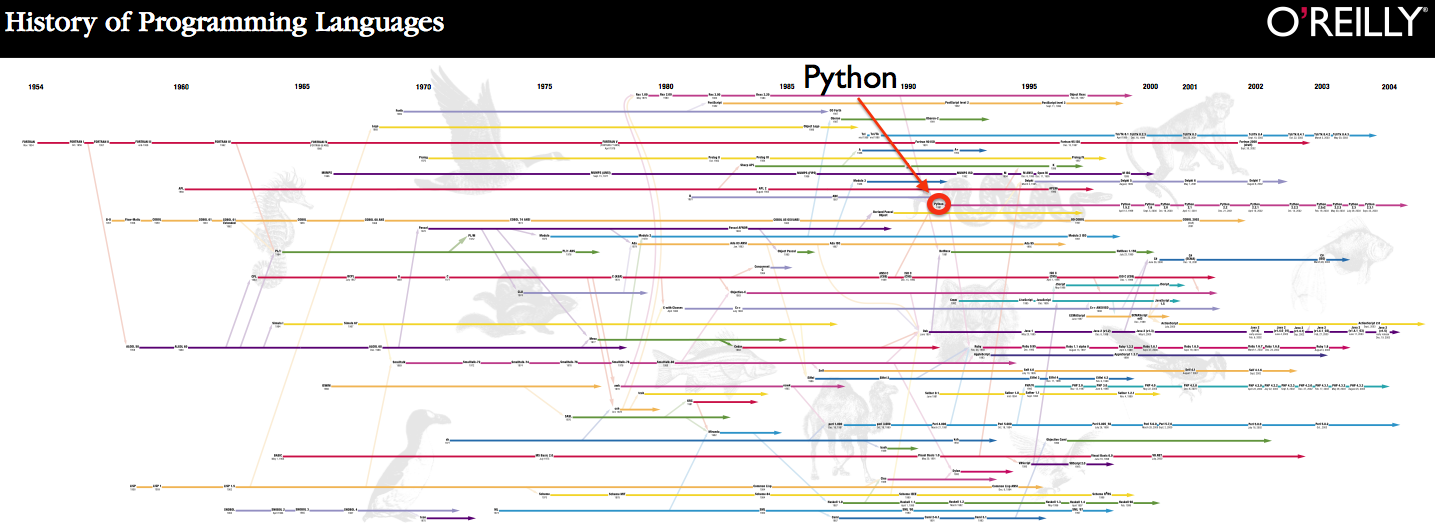
\includegraphics[width=305px]{ProgrammingLanguagesPoster-AnnotatedCropped.png} \\
    \tiny 
    Image credit: O'Reilly (\href{http://oreilly.com/news/graphics/prog\_lang\_poster.pdf}{http://oreilly.com/news/graphics/prog\_lang\_poster.pdf})
  \end{center}
\end{frame}

\begin{frame}
  \frametitle{Thanks!}
  \begin{itemize}
    \item We hope this little taste of the joys of programming whetted your appetite -- if so, this is the best place in the world to be.
    \item If you have any questions about Python, programming, or computer science in general, feel free to email either of us.
    \item Anshul: \href{mailto:anshul@gmail.com}{anshul@gmail.com}, Rob: \href{mailto:rpt@stanford.edu}{rpt@stanford.edu}.
    \item \texttt{\textbf{print 'Farewell, and godspeed!'}}
  \end{itemize}
\end{frame}



\end{document}
